%%%%%%%%%%%%%%%%%%%%%
% Experiments and Results %
%%%%%%%%%%%%%%%%%%%%%

This thesis aims to analyze the relationships between different road networks and road network similarity methods. In particular,  (1) the similarities between different road networks are determined, (2) similar road networks are clustered, (3) the correlations between the different network similarity methods used to identify the similarities between the different road networks are also determined, and (4) the similar methods are clustered. Figures \ref{fig:Road Network Similarity and Ranking} and \ref{fig:Road Network Similarity Method Correlation} show a high-level overview of the process. 

\begin{figure}[h]
\centering
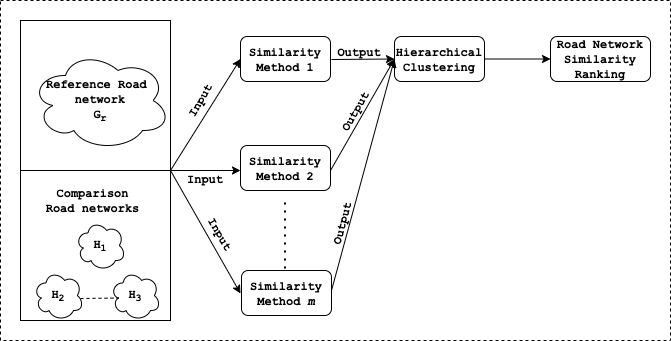
\includegraphics[width=0.75\textwidth,center]{picture/network_ranking.png}
\caption[Road Network Similarity and Ranking]{Road Network Similarity and Ranking}
\label{fig:Road Network Similarity and Ranking}
\end{figure}

\begin{figure}[!ht]
\centering
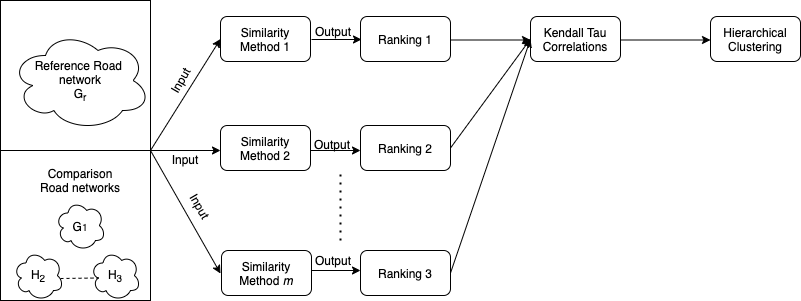
\includegraphics[width=0.75\textwidth,center]{picture/ranking.png}
\caption[Road Network Similarity Method Correlation]{Road Network Similarity Method Correlation}
\label{fig:Road Network Similarity Method Correlation}
\end{figure}


\section{Grid Road Network Similarity Analysis}
This section describes the experiments to identify similar road networks with Grid road network patterns and structure, likewise groups of methods described in Chapter 3 that have similar behavior.

The problem to find road networks with similar structures and patterns is explicitly approached using network-similarity ranking[Soundarajan]. Firstly, a reference network Gr and a collection of comparison networks H1, H2,...., Hk are given. A network-similarity method is used to calculate the similarity between Gr and each Hi. The data (similarity scores) for each comparison are normalized for uniformity before being used to create a dendrogram. This will cancel out the effects of outliers and ensure that the results have the same units. In Table 4.1 that shows the similarity score for each comparison, the normalization is accomplished by calculating Z scores for each similarity score in each column: z = (x mean)/std. As a result, the column mean is subtracted from each value in the column and then divided by the standard deviation. As a result, all the columns have the same mean and variance. The normed values indicate how many standard deviations any individual value deviates from the column mean. The hierarchical clustering algorithm can now be used in conjunction with the Ward variance minimization algorithm by combining the linkage function to generate the dendrogram. 

For the Grid road similarity analysis, the District of Columbia (USA) is selected as the reference network, then the methods are used to compare the other networks relative to the reference network and generate a numerical similarity score. This is followed by hierarchical clustering on the networks. Here, the interest is to learn whether certain road networks are similar to the refernce network, which generates a dendrogram displaying road network patterns that are similar to the reference road network pattern. The results for this analysis are presented in Figure \ref{fig:Hierarchical Clustering Dendrogram for Grid Road Networking Similarity}.

\begin{figure}[!ht]
\centering
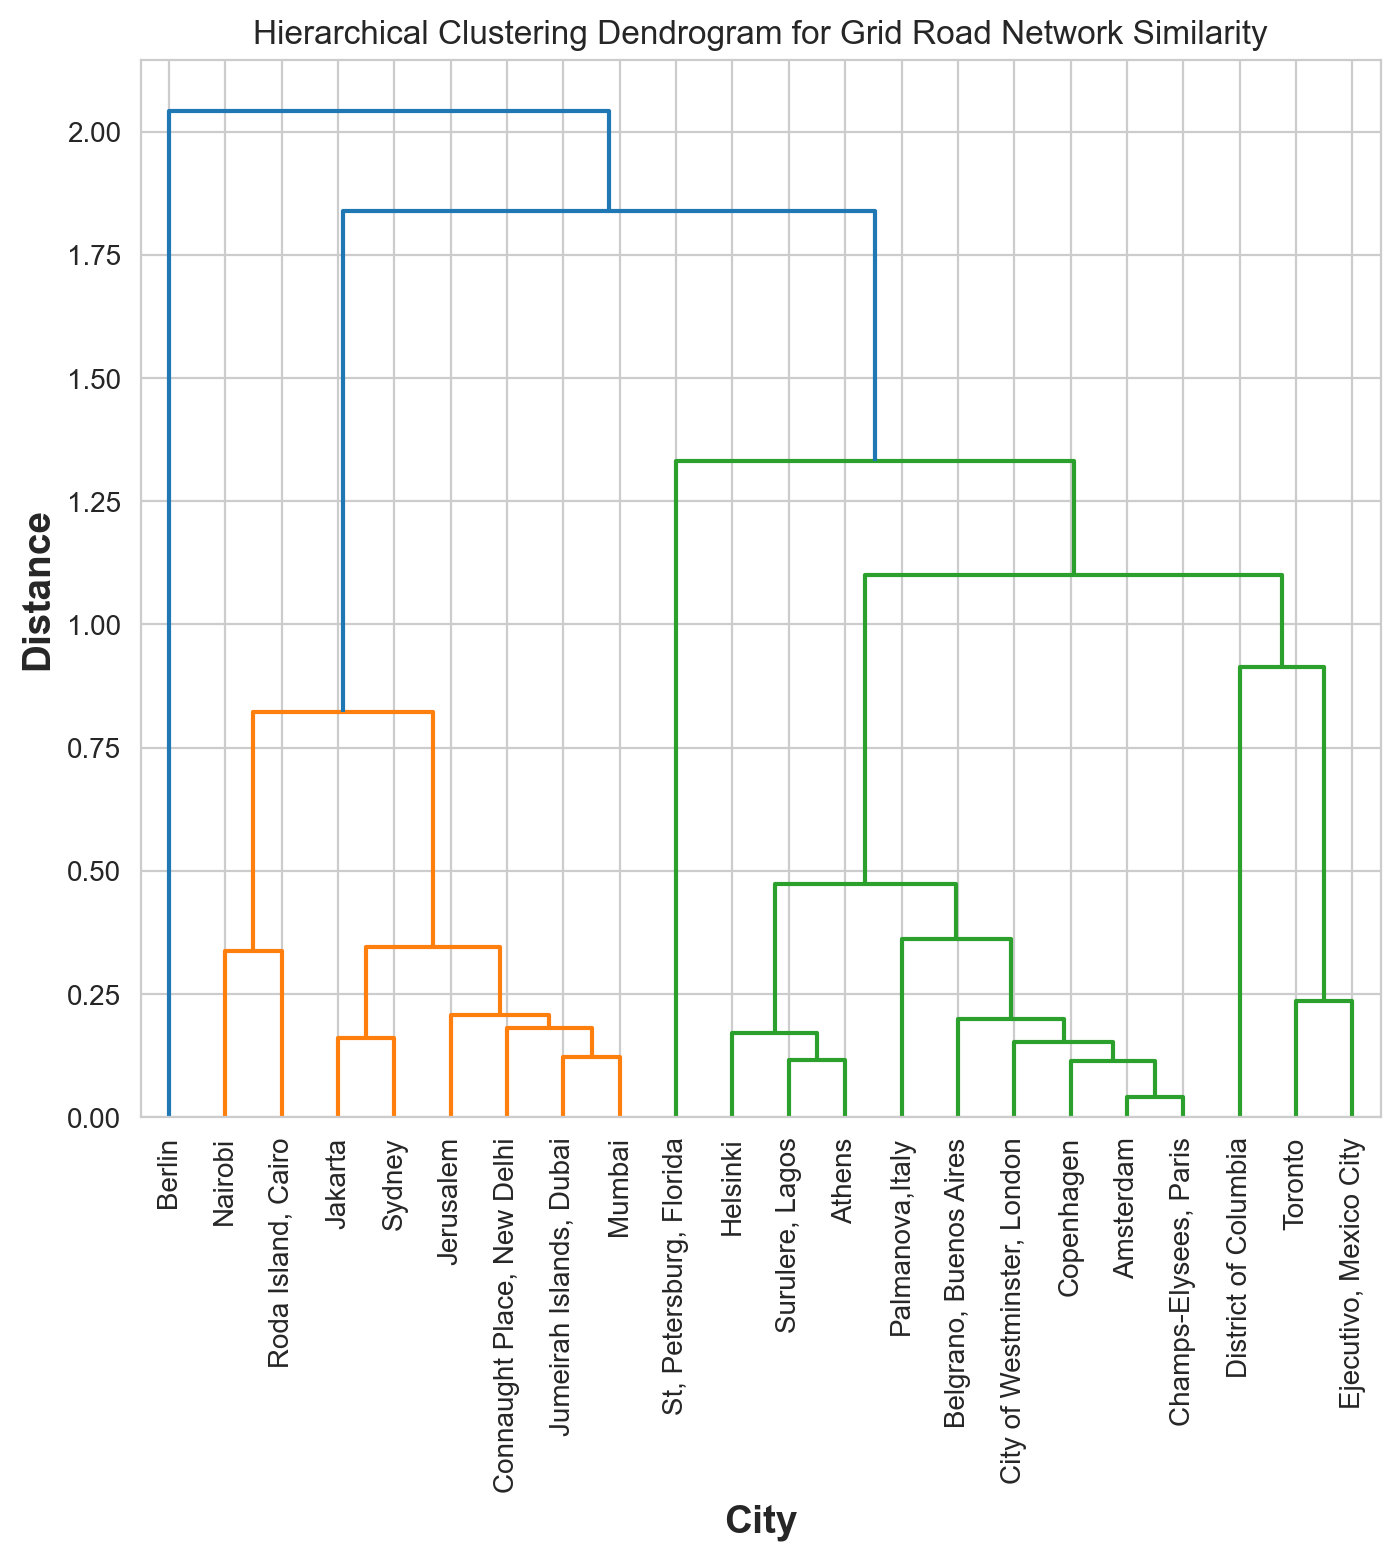
\includegraphics[width=0.75\textwidth,center]{picture/Grid/grid_dendrogram2.png}
\caption[Hierarchical Clustering Dendrogram for Grid Road Networking Similarity]{Hierarchical Clustering Dendrogram for Grid Road Networking Similarity}
\label{fig:Hierarchical Clustering Dendrogram for Grid Road Networking Similarity}
\end{figure}

Figure \ref{fig:Hierarchical Clustering Dendrogram for Grid Road Networking Similarity} presents the dendrogram obtained from the cluster analysis. From the dendrogram's structur,e 2 major clusters (Green and Orange) can be observed except for the outlier for the berlin road network (Blue). Each cluster contains road networks that are similar to one another. For example in the green cluster, the road network for the cities Ejecutivo and Toronto lie near the reference network: District of Columbia (USA) in one adjacent cluster which indicates that this cities have a pronounced grid-like structure similar to the reference network. 

However, the distance i Other cities include St, Petersburg Florida, hELSINKI, . Same is also evident for the cities Champs-Elysses, Paris, Amsterdam, Copenhagen.  In general, the overall distances between the clusters are not that large, and with some notable exceptions, the variations within the clusters are relatively small. By cross-checking with the similarity scores included in the heatmap in figure 4.4, it is possible to identify the characteristics of the 2 main groups and why certain groups belong to a cluster. 

\begin{figure}[!ht]
\centering
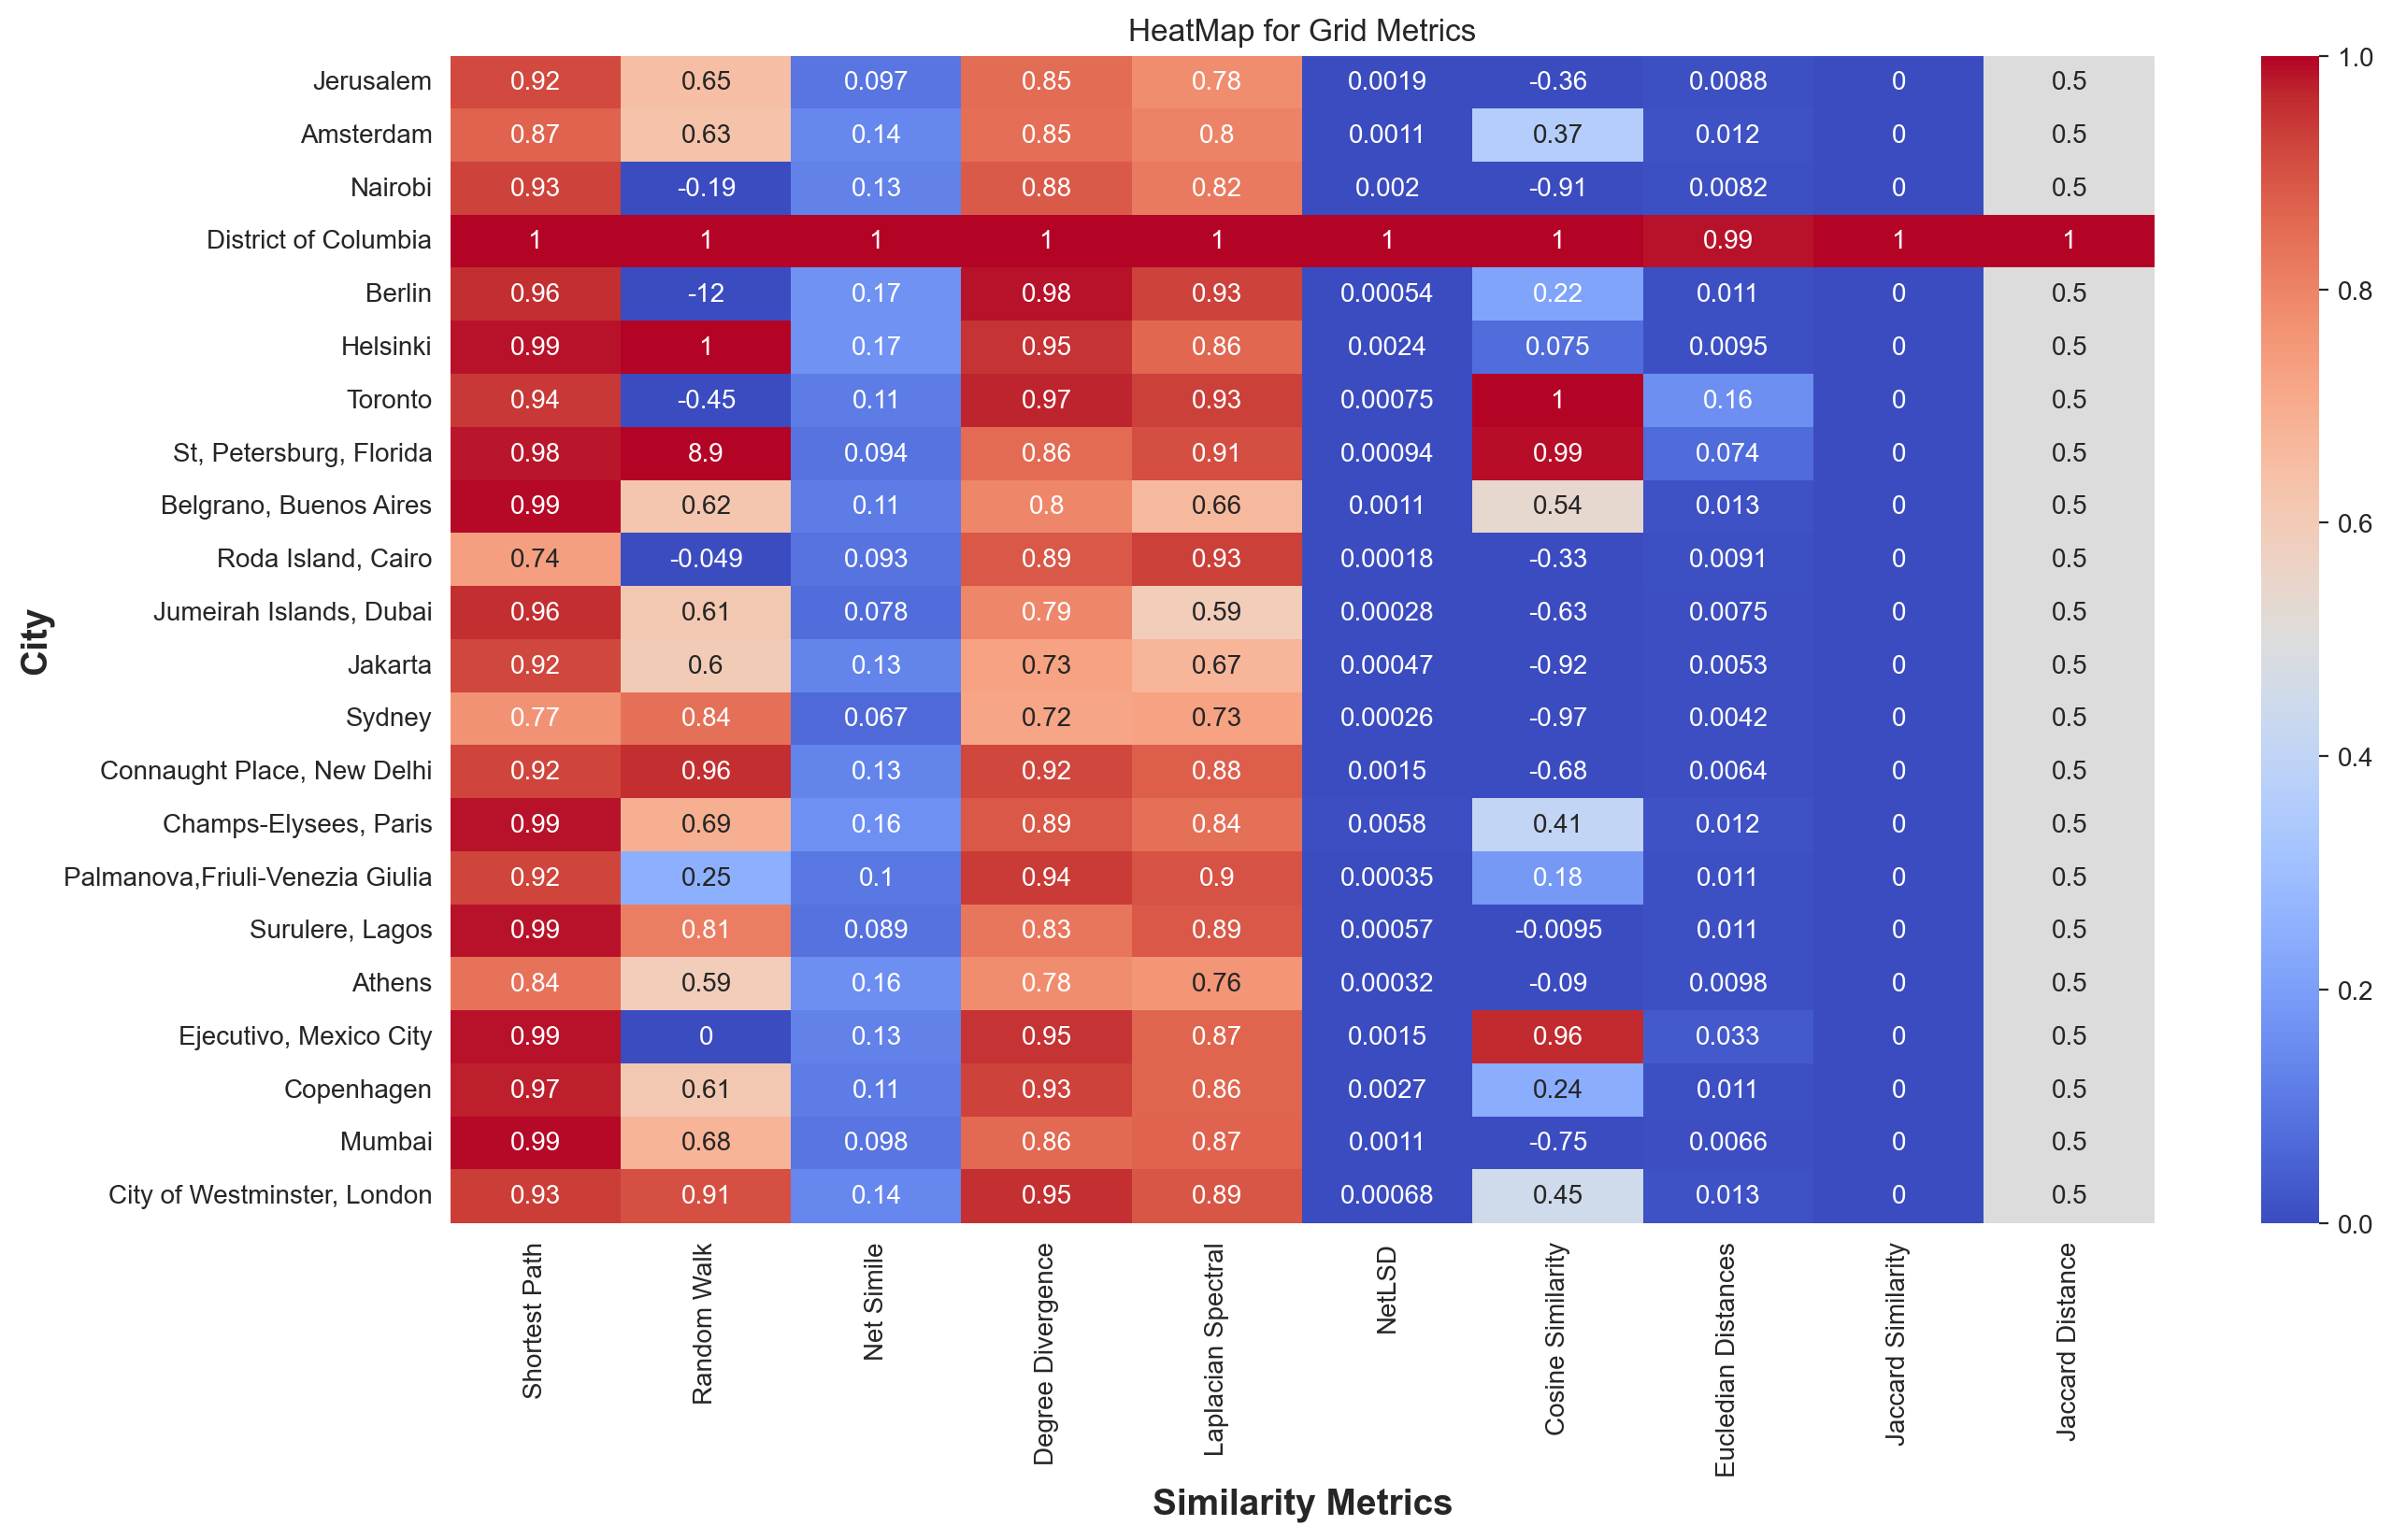
\includegraphics[width=0.85\textwidth,center]{picture/Grid/gridheatmap.png}
\caption[Heatmap showing the Kendall-Tau correlations for Grid Road Networks]{Heatmap showing the Kendall-Tau correlations between the road networks when the road network: District of Columbia was used as the reference network.}
\label{fig:Heatmap showing the Kendall-Tau correlations for Grid Road Networks}
\end{figure}

Ejecutivo and Toronto lie near the reference network in two adjacent clusters which contain grid-like—and almost exclusively North American—cities. The orange cluster represents relatively dense, gridded cities like Chicago, Portland, Vancouver, and Manhattan. The orange cluster contains less-perfectly gridded cities, typified by Sydney and New Delhi (plus, interestingly, Buenos Aires). The red cluster represents sprawling but relatively low-entropy cities like Los Angeles, Phoenix, and Las Vegas. Sprawling, high-entropy Charlotte is in a separate cluster (alongside Honolulu) dominated by cities that developed at least in part under the auspices of twentieth century communism, including Moscow, Kiev, Warsaw, Prague, Berlin, Kabul, Pyongyang, and Ulaanbaatar. Beijing and Shanghai are alone in their own cluster, more dissimilar from the other study sites. The dark gray cluster comprises the three cities with the most circuitous networks: Caracas, Hong Kong, and Sarajevo. While the US cities tend to group together in the red, orange, and blue clusters, the other world regions’ cities tend to distribute more evenly across the green, purple, and light gray clusters.

The first cluster (green in Figure 4.3) consists of the countries with the similar patterns to the to the reference network, with both district of Columbia and St,Petersburg, Florida standing out as outliers in terms of their distances. The result for this cluster is expected as DC was compared against itself with the value of the distance almost 
The second cluster is made up of wealthy and mostly urbanized countries. Luxembourg stands out as a singleton.
The red cluster contains the majority of the countries: they are neither very rich nor populous. A group of countries with the lowest levels of urbanization can be noted at the bottom of the chart.

Figure 4(a) presents the dendrogram of all of our networks built by hierarchical agglomerative clustering with unweighted
average linking. The network names are labelled on the x-xis. As evident in Figure 4(a), there is a
clear distinction between the clusters. The comparative networks with similar patterns to the reference network appear all together, along with other networks. The Oregon AS forms a cluster that only at the height of 0.45 joins with the Query Log. The Erd os-R enyi and Watts-Strogatz form a separate cluster. This, in turns, reflects our aforementioned intuition about following our background knowledge of the data. Similar results are obtained by applying the x-means clustering on the vectors of local features, for which we report the outcome in Table III. A part from the
distribution of the random networks, the clusters reflect what we observe in Figure 4(a).
Figure 4(b) shows the dendrogram for the above experiment (hierarchical agglomerative clustering with unweighted
average linking and the Canberra Distance) for graph vectors
generated by EIG. This figure clearly shows a different
picture, where the networks are grouped differently (see how
the distribution of the colors is mixed). For example, in the
leftmost cluster, two collaboration networks from arXiv are
put together with four Query Log networks, while the missing
Query Log network is placed together with the Oregon AS
networks. The EIG results are not intuitive, thus making EIG
not suitable for interpreting graph-similarity results.


This suggests that for frequent network similarity tasks,
one could use the computationally more efficient Density
method as a replacement for these computationally
intensive community-based methods.
Lastly, we apply the Kemeny-Young method to obtain
a single consensus ranking. Table 5 lists the five
similarity methods that are closest to this consensus for
each network, as measured by Kendall-Tau distance.
NetSimile (or one of its variations) and RWR appear
in the top five positions for each network. RWR has
an average Kendall-Tau distance of 0.06 from the consensus,
averaged over all networks. However, RWR has
an average Kendall-Tau distance of 0.21 from the other
similarity methods. This suggests that it is consistently
close to the consensus (i.e., median) ranking, but not
because it is simply close to the other rankings in general.
A user interested in selecting a single representative
method for network similarity ranking should thus
simply select NetSimile or RWR.



To find methods that behave similarly, Firstly, the pairwise Kendall-Tau distance between each pair of methods is calculated to determine correlations between the different methods which is then followed by a complete-linkage hierarchical clustering because it produces a dendrogram with many small clusters, which provides insight into which groups of methods are closely correlated—the results of this clustering show which groups of methods have similar behavior. 


\begin{figure}[!ht]
\centering
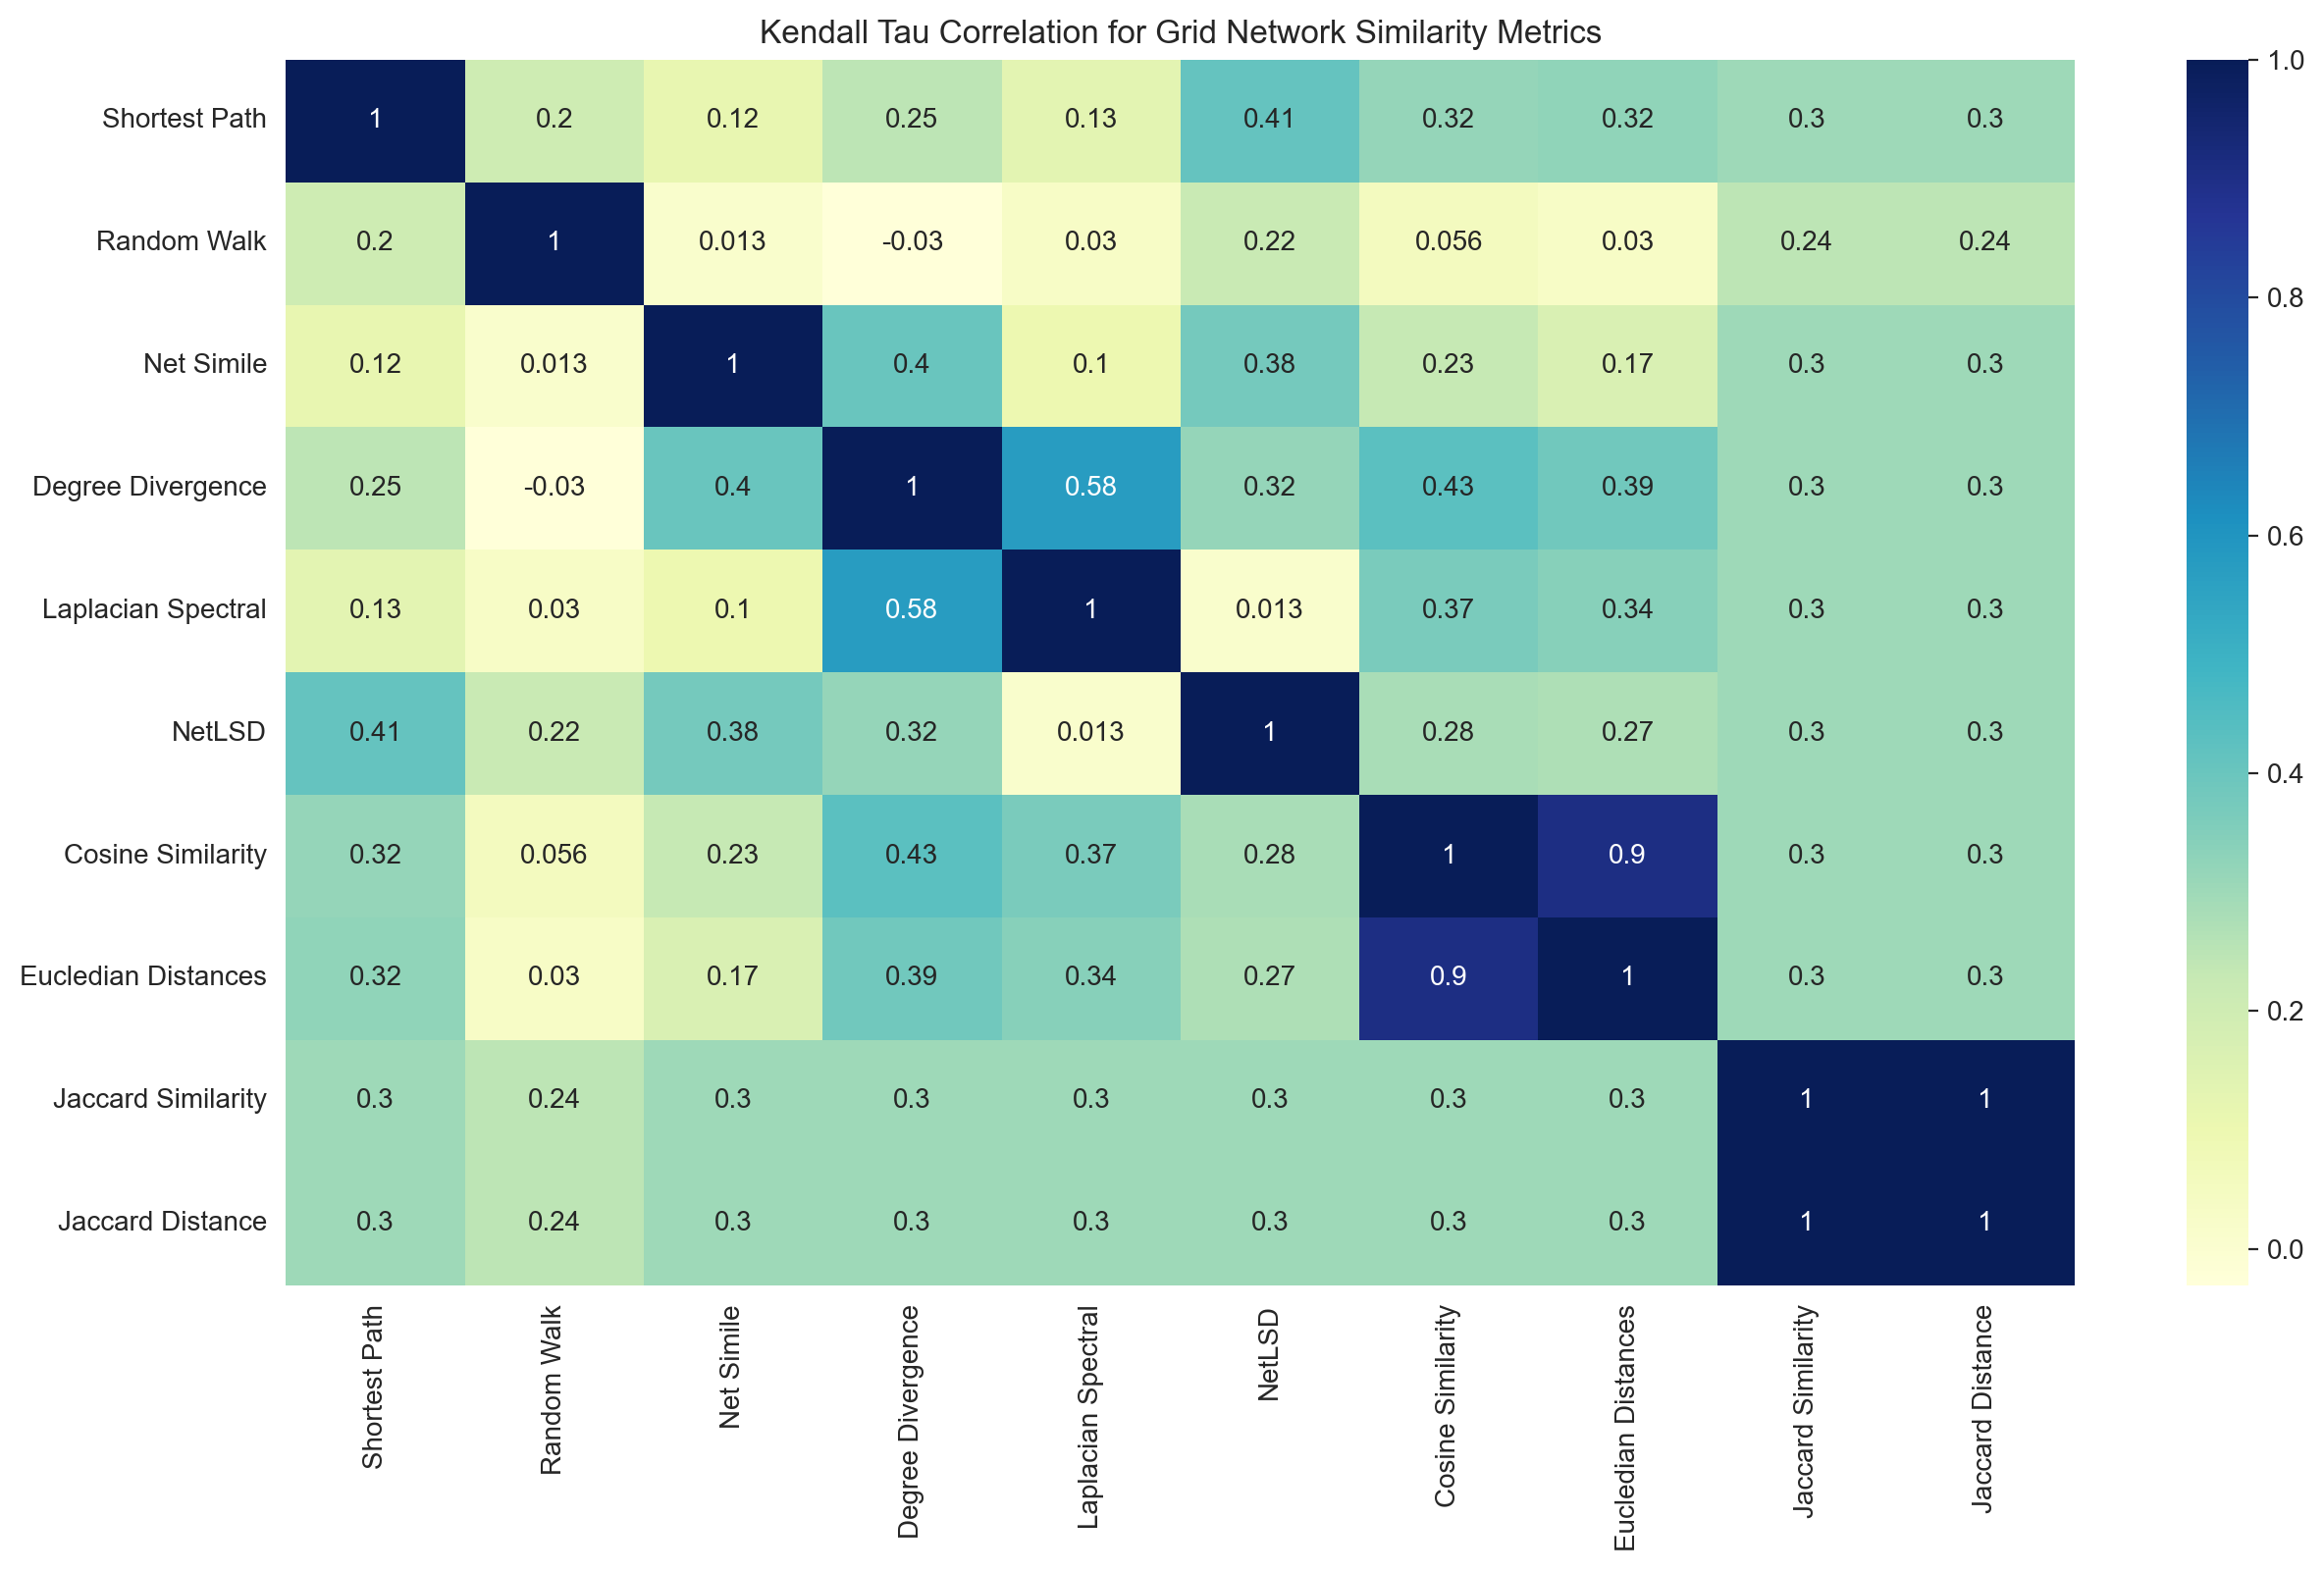
\includegraphics[width=0.85\textwidth,center]{picture/Grid/grid2.png}
\caption[Heatmap showing Kendall-Tau correlations between the road network similarity methods for Grid Road Networks]{Heatmap showing Kendall-Tau correlations between the road network similarity methods when the road network: District of Columbia was used as the reference network.}
\label{fig:network ranking}
\end{figure}

\begin{figure}[!ht]
\centering
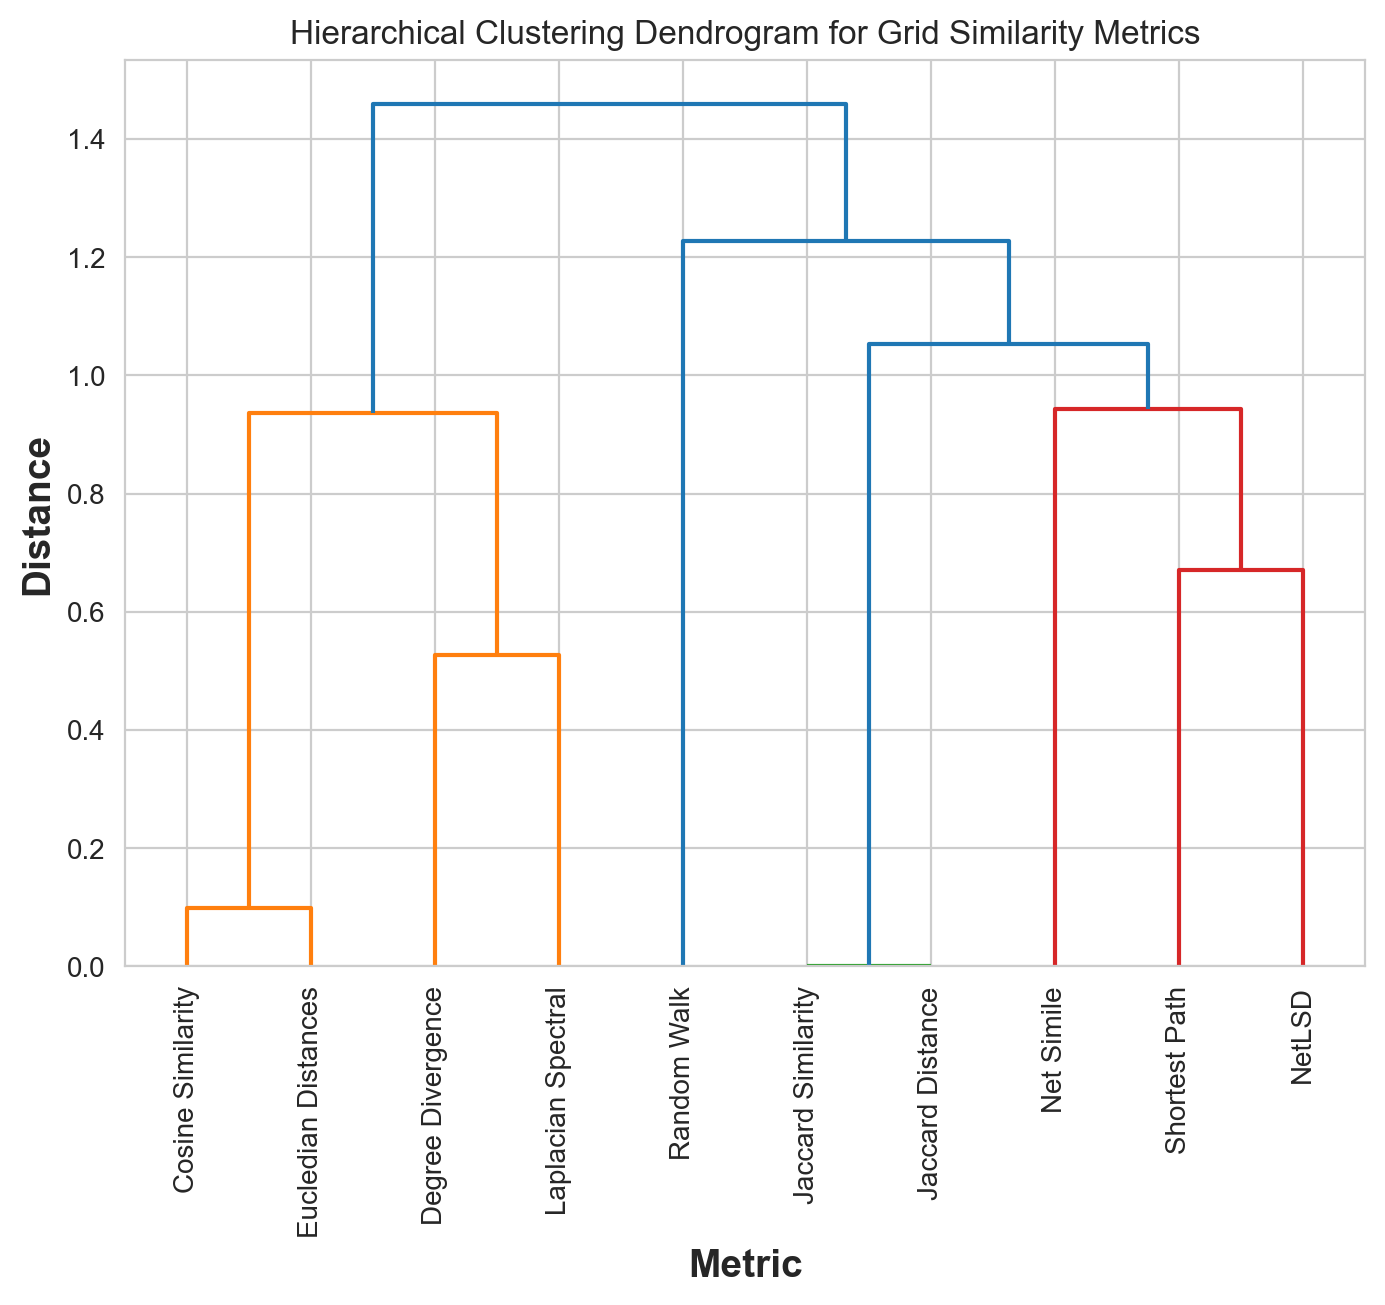
\includegraphics[width=0.85\textwidth,center]{picture/Grid/grid_metrics_dendrogram.png}
\caption[Hierarchical Clustering Dendrogram of the Correlation between the Road Network Similarity Methods for Grid Road Networks]{Hierarchical clustering dendrogram of the correlation between the road network similarity methods used to identify similar Grid road networks}
\label{fig:Hierarchical Clustering Dendrogram of the Correlation between the Road Network Similarity Methods for Grid Road Networks}
\end{figure}

Each square shows the correlation between the variables on each axis. Correlation ranges from -1 to +1. Values closer to zero means there is no linear trend between the two variables. The close to 1 the correlation is the more positively correlated they are; that is as one increases so does the other and the closer to 1 the stronger this relationship is. A correlation closer to -1 is similar, but instead of both increasing one variable will decrease as the other increases. The diagonals are all 1/dark green because those squares are correlating each variable to itself (so it's a perfect correlation). For the rest the larger the number and darker the color the higher the correlation between the two variables. The plot is also symmetrical about the diagonal since the same two variables are being paired together in those squares.

\section{Radial Road Network Similarity Analysis}
\begin{figure}[!ht]
\centering
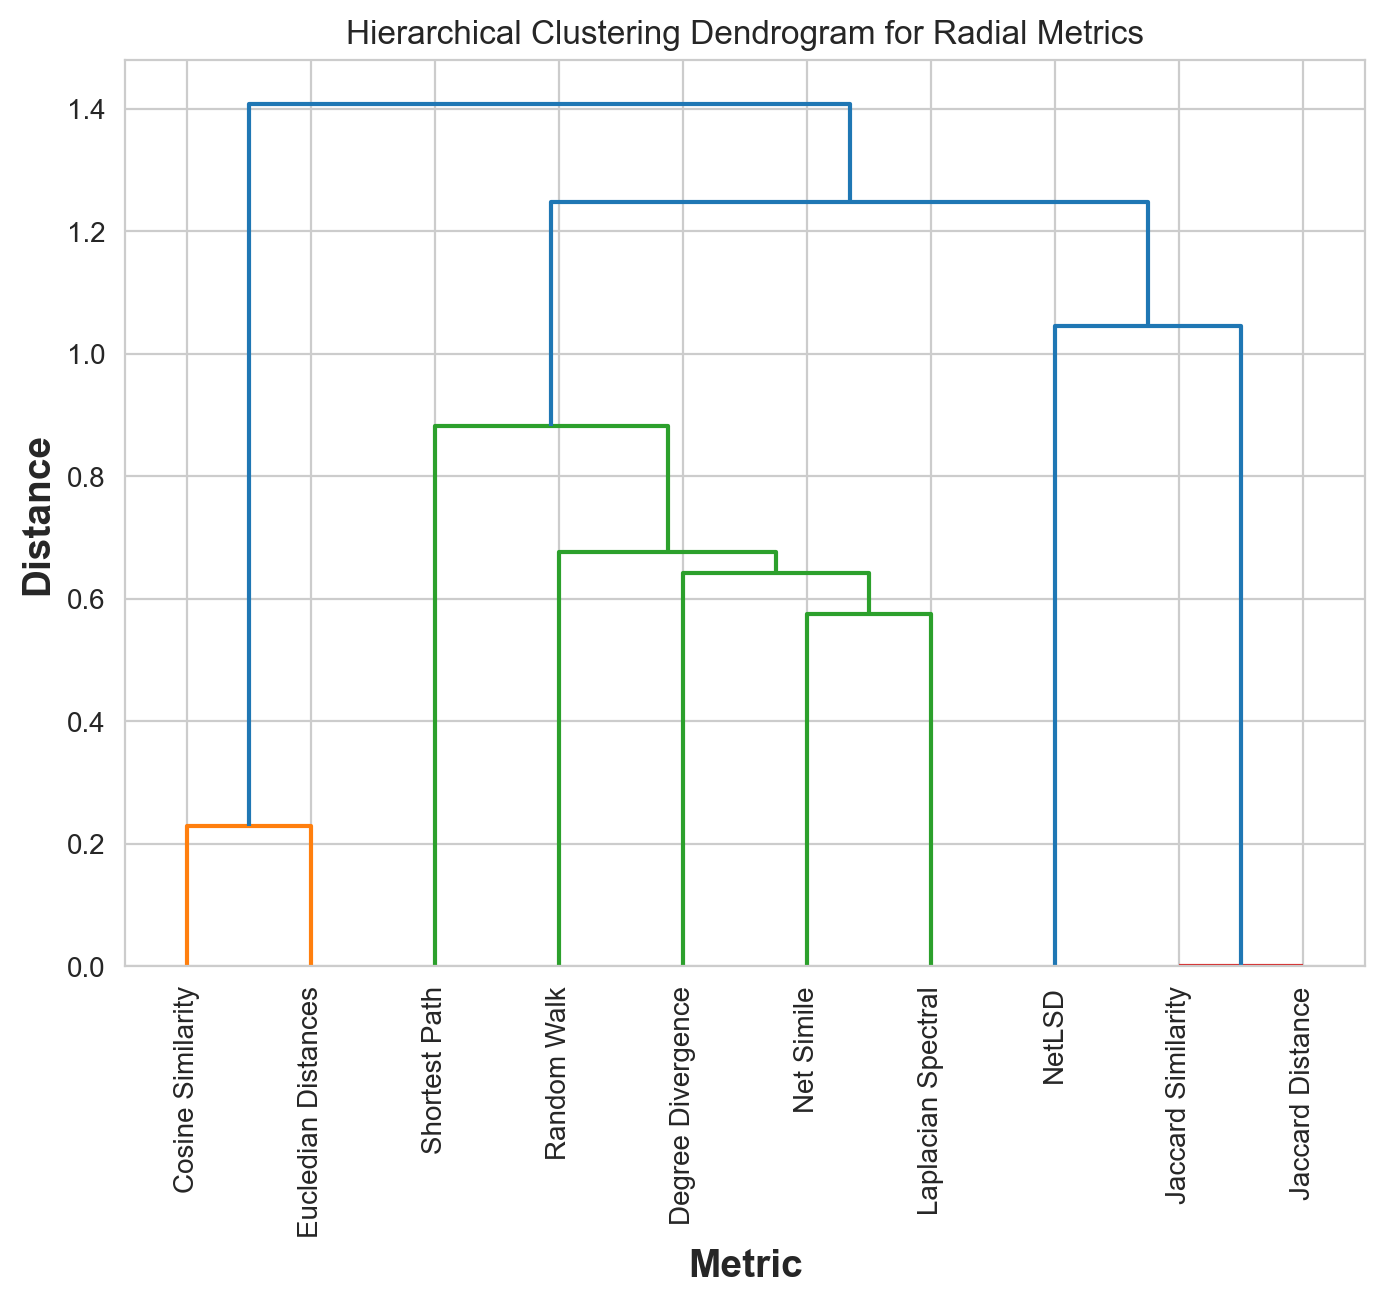
\includegraphics[width=0.85\textwidth,center]{picture/Radial/radial_metrics_dendrogram.png}
\caption[Hierarchical Clustering Dendrogram for Radial Road Networking Similarity]{Hierarchical Clustering Dendrogram for Radial Road Networking Similarity}
\label{fig:Hierarchical Clustering Dendrogram for Radial Road Networking Similarity}
\end{figure}

\section{Tree Road Network Similarity Analysis}
\section{Linear Road Network Similarity Analysis}
\section{Cul de Sac Road Network Similarity Analysis}
